\documentclass[11pt]{article}
\usepackage[margin=1in]{geometry}
\usepackage{titlesec}
\usepackage{url}
\usepackage{hyperref}
\usepackage{amsmath}
\usepackage{enumitem} % in preamble
\usepackage{graphicx}
\usepackage{float}
\usepackage{array}
\usepackage{pdflscape}
\usepackage{tabularx}


\graphicspath{{../Screenshots/}}
\setlist[itemize]{leftmargin=*, nosep, topsep=0pt, partopsep=0pt}

\newcommand{\memoheader}[4]{
  \noindent
  \textbf{From:} #2\\ 
  \textbf{To:} #1\\
  \textbf{Date:} #3\\
  \textbf{Subject:} #4\\[1ex]\hrule\vspace{1.5ex}


}




% --- Figure insertion helper ---
% This command simplifies inserting a figure with a caption and label.
% Usage: \insertfigure{width}{filename}{caption text}{fig:label}
%
% Parameters:
%   #1 = width relative to text width (e.g., 0.8 for 80%)
%   #2 = filename (without path if images are in the same directory)
%   #3 = caption text
%   #4 = label for cross-referencing (use fig: prefix by convention)
\newcommand{\insertfigure}[4]{%
    \begin{figure}[H] % figure in latex is a floating environment, H specifies to place figure specifically "Here"
        \centering
        \includegraphics[width=#1\textwidth]{#2}
        \caption{#3}
        \label{#4}
    \end{figure}
}






\begin{document}
\memoheader{Prof. Susan Gentry}
            {Miguel Cuaycong}
            {\today}
            {EMS 164: Simulation Memo 2}


\section{Background and Theory}
Thoroughly explains the motivation
and the specific physical factors (e.g.,
interfacial and strain energies)
considered in the model. Language is
accessible to an ENG 45 student,
clearly answering "Why do we care?"
\section{Key Methods of Paper}
Accurately and clearly describes the
specific analytical or experimental
methods used in the reference paper
to study the precipitates. This should
not only identify the test methods, but
briefly explain them.
\section{Key Findings of Paper}
Clearly summarizes the paper's
findings regarding the
expected/observed precipitate shape
and crystallography, using precise
and appropriate metallurgical
terminology.
\section{Test Method}
Concisely details the simulation setup
and all inputs needed to replicate the
study. No code is included in
document
\section{Simulation Results}
Results are accurate and presented
via clear, labeled figures and tables.
Simulation results are accurate based
on the input parameters.
% Required packages in preamble:
% \usepackage{tabularx}
% \usepackage{graphicx}

\begin{table}[htbp]
    \centering
    \renewcommand{\arraystretch}{1.5}
    \begin{tabularx}{\textwidth}{|>{\hsize=0.5\hsize}X|>{\hsize=1.0\hsize}X|>{\hsize=1.5\hsize}X|}
        \hline
        \textbf{Input Values} & \textbf{Outputs} & \textbf{Shape of Precipitate} \\
        \hline

        % --- Row 1 ---
        $\epsilon(1,1)$: \newline
        $\epsilon(2,2)$: \newline
        $\gamma(1,1)$:   \newline
        $\gamma(2,2)$:
        &
        Length 1:       \newline
        Length 2:       \newline
        Aspect Ratio:   \newline
        Volume Fraction:
        &
        % Replace with: \includegraphics[width=0.9\linewidth]{your-figure-1}
        \fbox{\parbox[c][4cm][c]{0.9\linewidth}{\centering FIGURE PLACEHOLDER}}
        \\
        \hline

        % --- Row 2 ---
        $\epsilon(1,1)$: \newline
        $\epsilon(2,2)$: \newline
        $\gamma(1,1)$:   \newline
        $\gamma(2,2)$:
        &
        Length 1:       \newline
        Length 2:       \newline
        Aspect Ratio:   \newline
        Volume Fraction:
        &
        \newline
        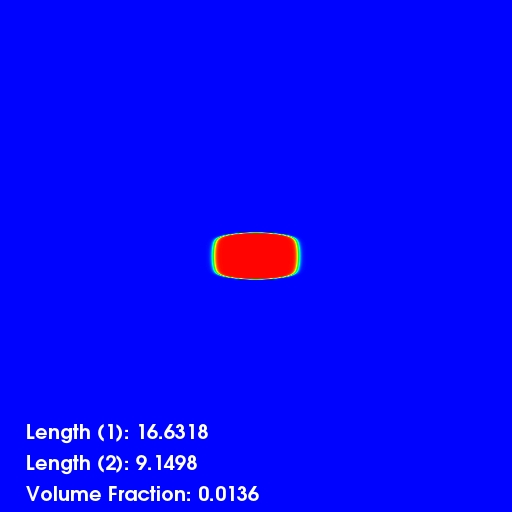
\includegraphics[width=\linewidth]{precipitateshape2.jpg}\\
        %\fbox{\parbox[c][4cm][c]{0.9\linewidth}{\centering FIGURE PLACEHOLDER}}
        \hline

        % --- Row 3 ---
        $\epsilon(1,1)$: \newline
        $\epsilon(2,2)$: \newline
        $\gamma(1,1)$:   \newline
        $\gamma(2,2)$:
        &
        Length 1:       \newline
        Length 2:       \newline
        Aspect Ratio:   \newline
        Volume Fraction:
        &
        % Replace with: \includegraphics[width=0.9\linewidth]{your-figure-3}
        \fbox{\parbox[c][4cm][c]{0.9\linewidth}{\centering FIGURE PLACEHOLDER}}
        \\
        \hline

    \end{tabularx}
    \caption{Simulation inputs, outputs, and shape of precipitate.}
    \label{tab:simulation}
\end{table}




\insertfigure{0.5}{precipitateshape1.jpg}{First precipitate shape PLACEHOLDER}{fig:precipitate1}
\insertfigure{0.5}{precipitateshape2.jpg}{Second precipitate shape PLACEHOLDER}{fig:precipitate2}
\insertfigure{0.5}{precipitateshape3.jpg}{Third precipitate shape PLACEHOLDER}{fig:precipitate3}
\section{Simulation Synthesis}
Directly answers the specific research
prompt using the simulation data.
Deeply connects the "what" (the
results) to the "why" by explicitly
referencing figures and tables in the
discussion.
\section{Comparison to literature}
Critically evaluates the simulation's assumptions 
against real-world experiments. Provides a thoughtful 
discussion on the physical limitations of the model.
\end{document}